\section{\bench}
\label{sec:bench}

We construct \textbf{\bench} to evaluate language world models across seven agent interaction domains.
When an LWM simulates environments, predicting each turn's observation requires comprehending the full interaction history accumulated across all prior turns.
As trajectories grow longer, maintaining fidelity to this context becomes increasingly challenging, making \bench a naturally grounded long-context benchmark.
Ensuring simulation quality further requires that a world-model benchmark verify whether predicted environment responses match reality across format, factuality, state consistency, and domain-specific conventions.

\subsection{Benchmark Construction}
\label{sec:bench:construction}

\bench is constructed from agentic trajectories of frontier models on established benchmarks across all seven domains, converted into environment trajectories (\S\ref{sec:prelim:schema}) with ground-truth observations obtained from the real environments.


\paragraph{Construction Principles.}
\bench is built on four construction principles:
(i)~\emph{Widely-Used Queries:} all task queries are drawn from established high-quality agentic benchmarks rather than self-constructed tasks, so that the task distribution aligns with the scenarios that current agent development targets;
(ii)~\emph{Frontier-Agent Trajectories:} all trajectories are generated by frontier-model agents, whose actions (long reasoning chains, tool-call compositions, and error-recovery sequences) are high-quality and sufficiently complex to stress-test world-model fidelity at the frontier scale;
(iii)~\emph{Real Observations:} every trajectory is paired with ground-truth observations from real environment execution, providing a reference for evaluation;
(iv)~\emph{Out-of-Distribution:} training data and benchmark queries are partitioned at the data-source level, so that \bench probes generalization rather than memorization;

\paragraph{Data Collection.}
Figure~\ref{fig:bench_overview} summarizes the source benchmarks and trajectory statistics for each domain.
We deploy 5 frontier agents on 9 established benchmark query sets across all 7 domains, execute them against real environments to produce agentic trajectories, and then extract environment trajectories (\S\ref{sec:prelim:schema}).
For text-based domains, an early subset (Terminal-Bench~1.0 and the in-house SWE benchmark) was collected with Claude Sonnet~4.5.
All remaining text-domain trajectories use Claude Opus~4.6 exclusively, ensuring that \bench evaluates whether an LWM can faithfully simulate environments to support the workflows of the most capable agents.
For GUI domains, we further diversify the agent pool by adding 3 strong Qwen-family models, expanding coverage to 5 frontier models and producing more varied action sequences for comprehensive evaluation.


\paragraph{Turn-level Sampling Strategy.}
\label{sec:bench:construction:turn_sampling}

Due to the large volume of raw agentic trajectories, we subsample the source trajectories for the in-house SWE benchmark and the 3 GUI benchmarks before applying the turn-level expansion described below.
When trajectories are expanded into turn-level evaluation samples, all text domains use an asymmetric sampling strategy: each trajectory keeps the first and last turns, plus three uniformly sampled intermediate turns, for five evaluation turns in total.
The first turn tests initial simulation without interaction history.
Errors at this turn propagate recursively through the state chain, so first-turn fidelity acts as an anchor.
The last turn has the longest context and the strongest dependence on accumulated prior state. It is the primary probe for long-context simulation fidelity.
The three intermediate turns provide broader coverage of mid-trajectory behavior (tool-call chaining, incremental state updates, error recovery) and dilute the boundary bias.
For GUI domains, since certain operations are overly simplistic (e.g., entering text into an input field), we selectively sampled the more challenging turns from the trajectories during the expansion process.
After the trajectory-to-turn expansion, we further retain a uniform 50\% random sample to form the final benchmark, balancing evaluation coverage against computational cost.

\paragraph{Benchmark Statistics.}
\label{sec:bench:construction:stats}
Figure~\ref{fig:bench_overview} shows the domain coverage and evaluation framework of \bench, which contains 2,170 evaluation samples in total.
The four text-based domains collectively account for 72.4\% of the benchmark, with SWE (21.8\%) and Search (21.1\%) contributing the largest shares, followed by Terminal (16.3\%) and MCP (13.2\%). The three GUI domains each contribute 9.2\%.
The average context length varies across domains: MCP samples average 59,300 tokens because each sample embeds the full tool-definition schema in its system prompt, whereas Terminal samples are the shortest at 12,900 tokens, reflecting self-contained shell sessions.

\begin{figure*}[t]
\centering
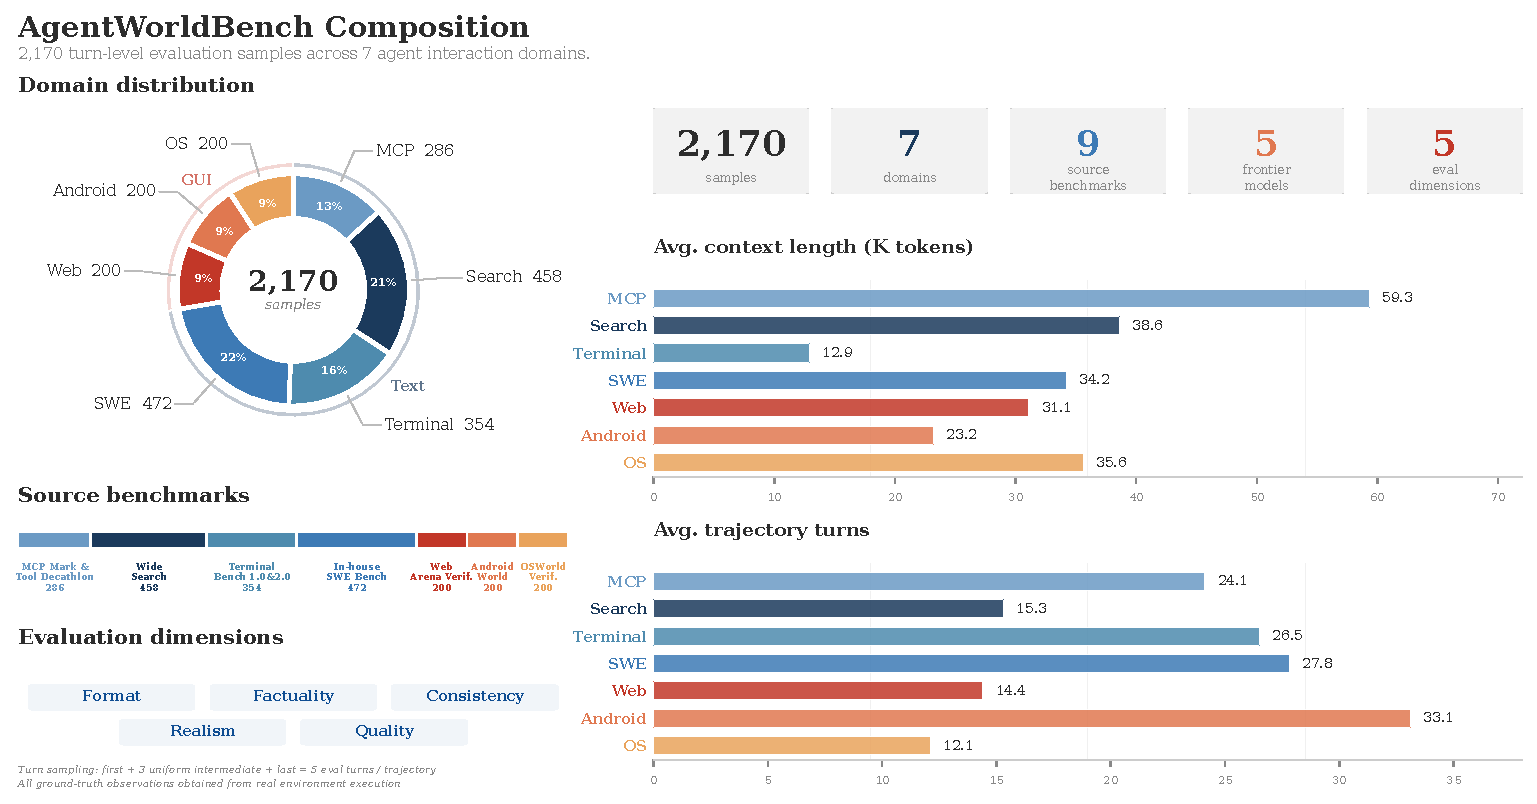
\includegraphics[width=\linewidth]{figures/bench_overview.pdf}
\caption{
    Overview of \bench composition.
    \textbf{Left:} Domain distribution across seven domains, source benchmarks mapped to each domain, and the five evaluation dimensions (Format, Factuality, Consistency, Realism, Quality).
    \textbf{Right:} Summary statistics, per-domain average context length and trajectory depth.
    All ground-truth observations are obtained from real environment execution.
}
\label{fig:bench_overview}
\end{figure*}

\subsection{Evaluation Protocol}
\label{sec:bench:protocol}

\bench evaluates simulation quality through an open-ended rubric: an LLM judge scores each predicted observation on five dimensions: \textbf{Format}, \textbf{Factuality}, \textbf{Consistency}, \textbf{Realism}, and \textbf{Quality}.
The primary score is the mean across the five dimensions, scaled to $[0, 100]$.
Format measures whether the output obeys the structural conventions of the domain (JSON schema compliance for MCP, shell prompt patterns for Terminal).
Factuality measures whether stated facts (file contents, search results, tool return values) are correct.
Consistency measures whether the output is internally coherent and coherent with prior turns.
Realism measures whether the simulation matches the behavioral characteristics of the real environment as evidenced by the ground truth, including response patterns, style conventions, and value plausibility.
Quality measures completeness and conciseness relative to the ground truth: critical information must not be omitted, and the output should not be excessively verbose or abbreviated compared to the reference.

\paragraph{Reference-Grounded Judging.}
The judge receives the ground-truth environment observation alongside the predicted observation and scores each dimension by comparing the two.
This reference-grounded design converts the evaluation from an open-ended quality judgment into a factual comparison, substantially narrowing the space for judge hallucination or misjudgment: the judge does not need to independently reason about what a correct environment response should look like, because the real output serves as an unambiguous reference.
This is also the primary reason for the high cross-judge consistency reported below: when scoring against a concrete reference rather than abstract quality criteria, different judge models converge on the same rankings.

\paragraph{Domain-Aware Rubrics.}
Each domain has its own judge prompt that applies the five dimensions in domain-specific terms, ensuring that evaluation not only compares against the reference objectively but also enforces the professional standards of each domain (full prompts in Appendix~\ref{sec:appendix:judge_prompts}).
For example, Terminal judges verify shell prompt patterns and cross-turn state tracking (working directory, environment variables, file-system mutations), MCP judges enforce JSON schema compliance and resource lifecycle consistency, Search judges apply a fact-priority hierarchy where contradicting the reference answer scores zero on Factuality regardless of surface plausibility, and SWE judges enforce tool execution correctness (success/failure status, exit codes) and file-system state persistence across turns.

\paragraph{Differentiated Matching Criteria.}
Not all content in an environment observation requires exact matching, and treating all content uniformly produces excessive false negatives.
We classify content into three types before evaluation.
\emph{Deterministic content} (echo output, file reads, computation results) must match exactly. A \texttt{cat} command that returns the wrong file contents is unambiguously wrong.
\emph{Pre-existing environment content} (preinstalled software versions, file contents not created by the trajectory) requires only format and plausibility verification, because a simulator cannot reproduce the exact patch version of \texttt{gcc} in a particular sandbox.
\emph{Runtime metadata} (timestamps, PIDs, memory addresses, session tokens) requires only format and range verification. A simulated PID of 42731 is as acceptable as the real 18204, provided both are valid.
This three-way split lets the judge reward correct structural and semantic behavior without penalizing irreproducible details.

\paragraph{Judge Selection.}
\label{sec:bench:judge}
We use a double-blind Turing test as a calibration tool to select the judge model and tune the judge prompt.
Given the interaction history up to a prediction turn and the current action, the judge receives two candidate observations in randomized order, one from the real environment and one from the world model, and must identify which came from the real environment.
We randomize the presentation order to control for position bias and use real observations rather than outputs from another world model to avoid distributional confounds.
The rationale is that a judge with high Turing-test accuracy must attend to fine-grained differences between faithful and plausible-but-wrong simulation, the same discriminative ability required for accurate rubric scoring.
We iteratively refine domain-specific judge prompts via autoresearch~\citep{karpathy2026autoresearch} using Turing-test accuracy as the optimization signal, analyzing per-domain error patterns to adjust rubric definitions, differentiated matching boundaries, and scoring anchors until the prompts achieve stable accuracy.

With calibrated prompts in place, we evaluate whether the choice of judge model affects evaluation outcomes.
We compare three frontier models as judge candidates, Gemini 3 Flash~\citep{gemini3flash}, Claude Sonnet 4.5~\citep{sonnet4.5}, and GPT-5.2~\citep{gpt-5.2}, by having each independently score predictions from all models in Table~\ref{tab:main_results} across all seven domains of \bench{}.
Absolute scores show a systematic spread: Gemini 3 Flash is the most lenient and GPT-5.2 the most stringent rater across all domains.
Despite these absolute differences, the model-level rankings are highly consistent across judges: the pairwise Spearman rank correlations are $\rho = 0.92$--$0.99$ (all $p < 10^{-5}$), indicating that the three judges agree on which models produce higher-fidelity predictions despite assigning different absolute scores.
The per-dimension ordering is also preserved: all three judges rank Format and Consistency as the two strongest dimensions while identifying Factuality as the weakest, with a shared ordering of Realism $>$ Quality $>$ Factuality across all judges.
We attribute this cross-judge ranking consistency to the reference-grounded design: each judge scores against the real environment output, reducing the task to factual comparison rather than subjective quality assessment.
Since the relative ranking is stable across judges, we select GPT-5.2 as the judge for its highest average Turing-test accuracy.
